\def\x{x}
\def\Q{Q}
\def\bds#1{#1}
\def\tts#1{\texttt{\small #1}}

\section{Experiments}
\label{sec:thesims}
%\subsection{Simulations}
We first illustrate our methods using a simulation of the model
\begin{equation}\nonumber
         Y_i = \x_{iS}^{\top}\Q\x_{iS} + \epsilon_i \quad (i=1,2,\ldots,n).
\end{equation}
Here $\x_{i}$ denotes data sample $i$ drawn from $\mathcal{N}(\bds{0}, \Sigma)$, 
$\x_{iS}$ is a subset of $\x_i$ with dimension $|S|=5$, where $S$
represents the relevant variable set, and 
$\epsilon_i$ is additive noise drawn from $\mathcal{N}(0,1)$. 
The matrix $\Q$ is a symmetric positive definite matrix of dimension $|S|\times{}|S|$. 
Note that if $\Q$ is diagonal, then the true function is convex
additive; 
otherwise the true function is convex but not additive.
For all simulations in this section, we set $\lambda=4\sqrt{{\log(np)}/{n}}$. 

In the first simulation, we vary the ambient dimension $p$. We set $Q$ as one on the diagonal and $1/2$ on the off-diagonal with $0.5$ probability, and choose $n=100, 200,\ldots,1000$ and $p=64,128,256$ and $512$. We use independent design by setting $\Sigma = \textrm{I}_p$.
For each $(n,p)$ combination, we generate $100$ independent data
sets. For each data set we use the AC/DC algorithm and mark feature $j$ as irrelevant if both the AC estimate $\| \hat{f}_j \|_\infty$ and the DC estimate $\| \hat{g}_k \|_\infty$ are smaller than $10^{-6}$.
We plot the probability of exact
support recovery over the $100$ data sets in Figure \ref{Support}(a).  We
observe that the algorithm performs consistent variable selection even if the dimensionality is large. To give the reader a
sense of the running speed, for a 
data set with $n=1000$ and $p=512$, the code runs in roughly two 
minutes on a machine with 2.3 GHz Intel Core i5 CPU and 4 GB memory.

In the second simulation, we vary the sparsity of the $Q$ matrix, that is, we vary the extent to which the true function is non-additive. We generate four $\Q$ matrices
plotted in Figure \ref{Support}(b), where the diagonal elements are all one and
the off-diagonal elements are $\frac{1}{2}$ with probability $\alpha$
($\alpha=0,0.2,0.5,1$ for the four cases). We fix $p=128$ and choose
$n=100,200,\ldots,1000$. We use independent design by seting $\Sigma = \textrm{I}_p$. We again run the AC/DC optimization on $100$
independently generated data sets and plot the probability of recovery
in Figure \ref{Support}(c). The results demonstrate that AC/DC performs
consistent variable selection even if the true function is not additive (but
still convex).

In the third simulation, we use correlated design and vary the correlation. We let
$\x_i$ be drawn from $\mathcal{N}(\bds{0},\bds{\Sigma})$
instead of $\mathcal{N}(\bds{0},\bds{I}_{p})$, with
$\Sigma_{ij}=\nu^{|i-j|}$. We use the non-additive $\Q$, same as in the second experiment, with $\alpha=0.5$ and fix $p=128$.  The recovery curves for $\nu=0.2, 0.4,
0.6, 0.8$ are shown in Figure \ref{Support}(d). As can be seen, for
design of moderate correlation, AC/DC can still select relevant
variables well.


%\begin{figure}[!htpb]
%        \centering
%        \begin{subfigure}[b]{0.45\textwidth}
%                \centering
%                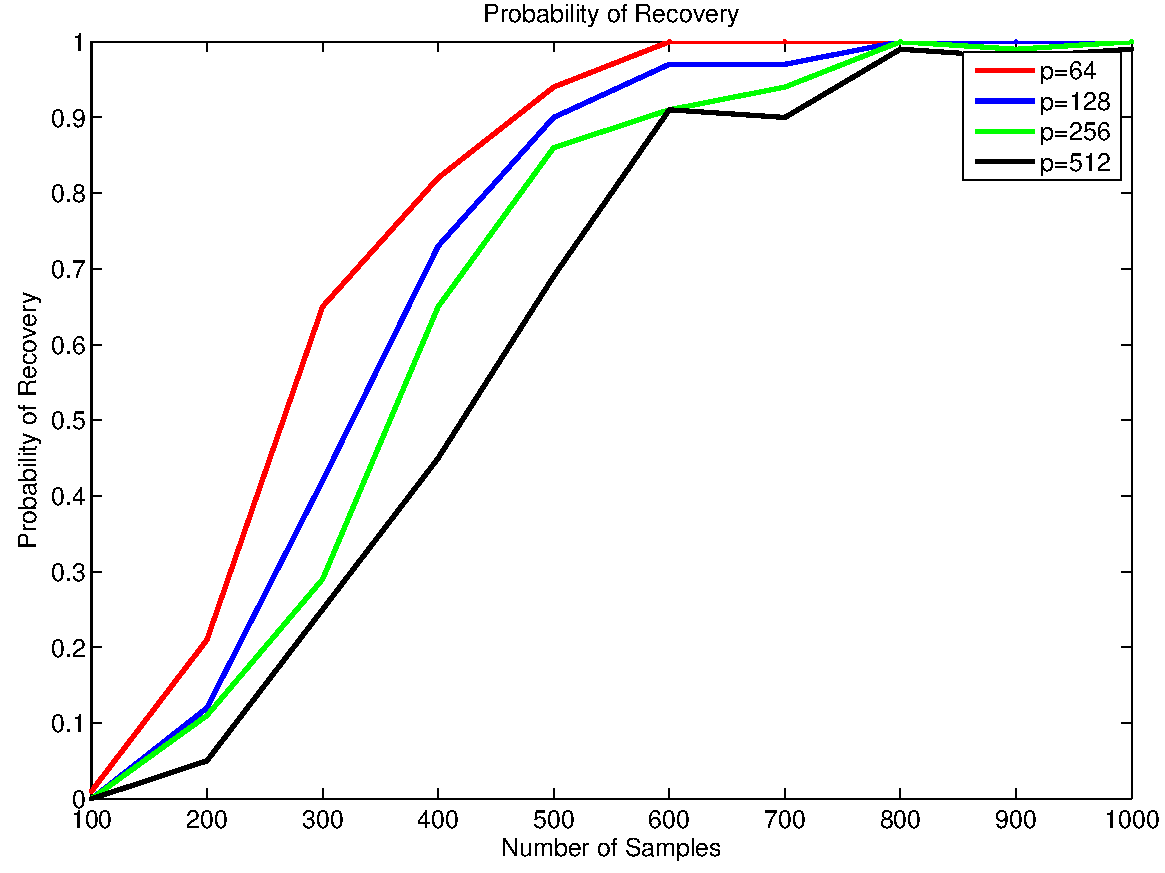
\includegraphics[width=\textwidth]{figs/Curve1}
%                 \caption{Additive model.}
%                \label{Curve1}
%        \end{subfigure}
%        \begin{subfigure}[b]{0.45\textwidth}
%                \centering
%                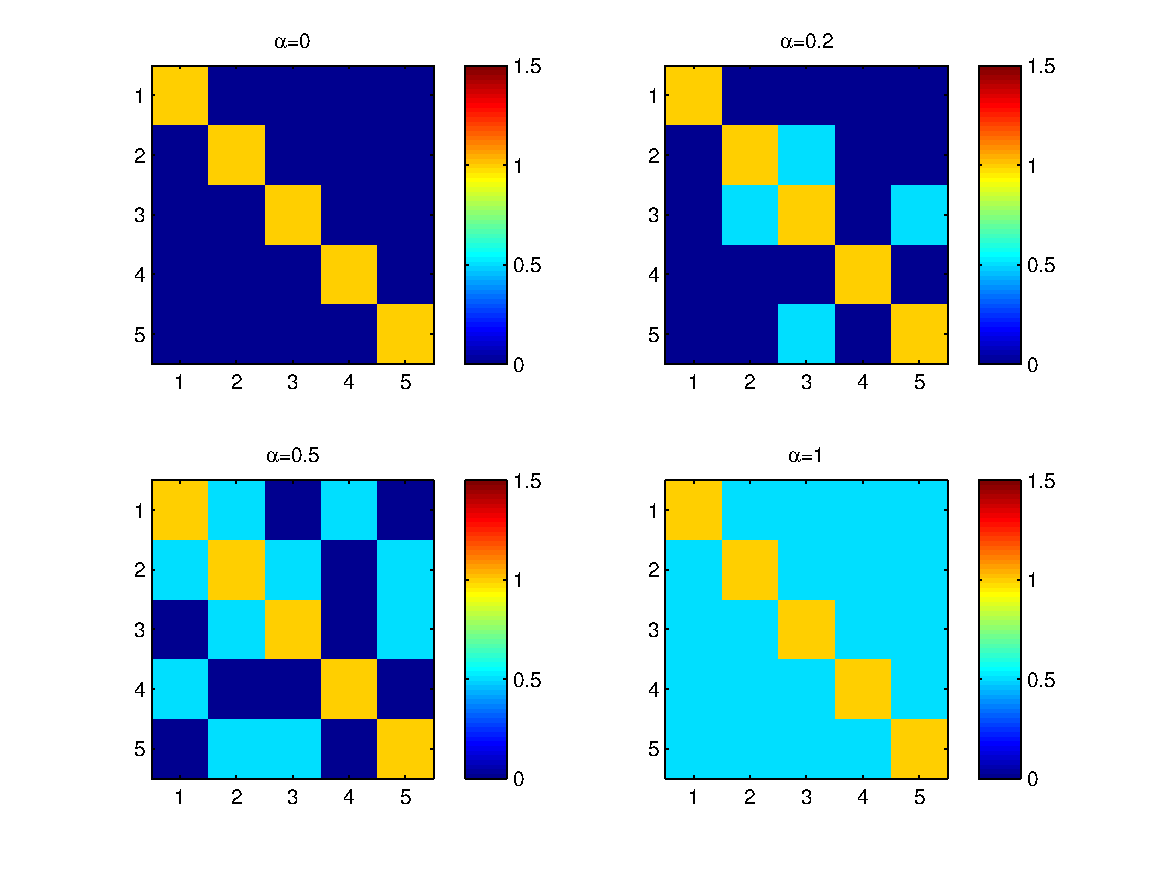
\includegraphics[width=\textwidth]{figs/Q}
%                \caption{Four $\Q$ matrices.}
%                \label{Q}
%        \end{subfigure}\\
%        \begin{subfigure}[b]{0.45\textwidth}
%                \centering
%                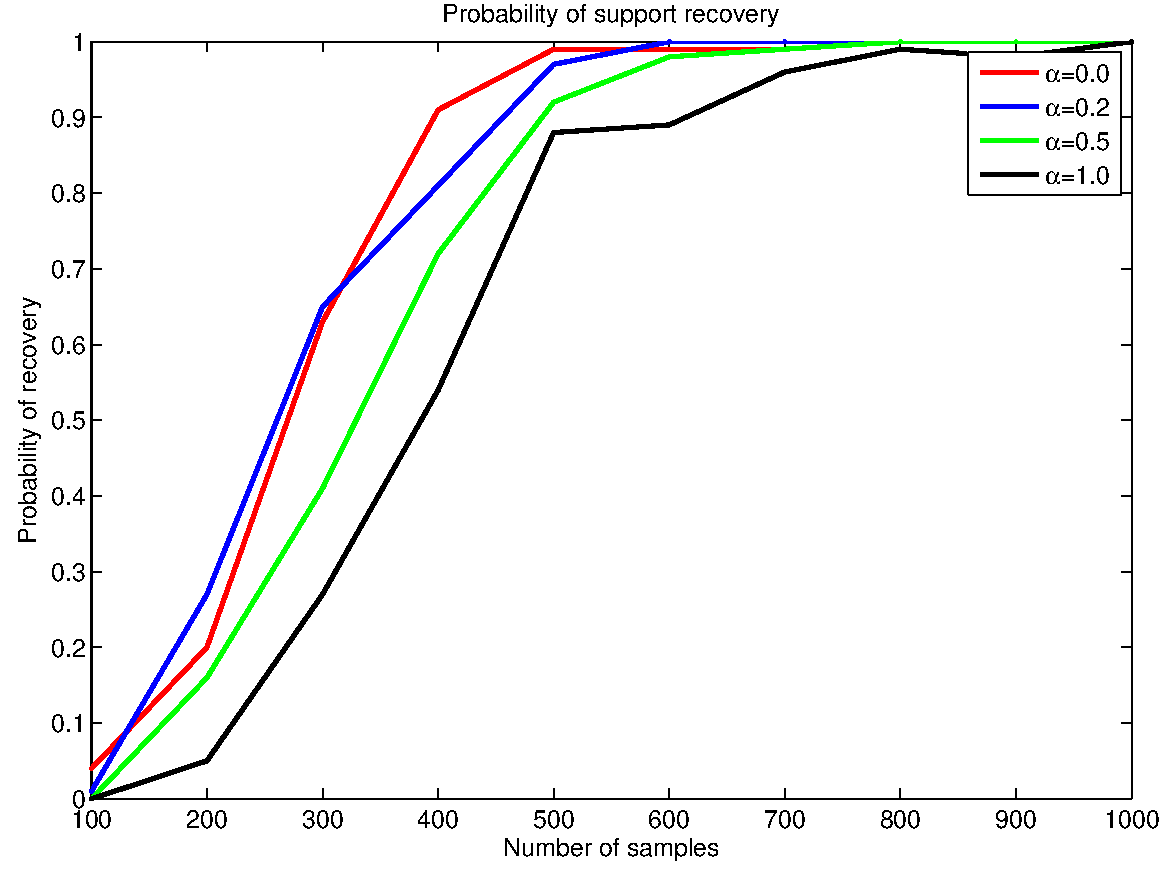
\includegraphics[width=\textwidth]{figs/Curve2}
%                \caption{Additive and non-additive models.}
%                \label{Curve2}
%        \end{subfigure}
%        \begin{subfigure}[b]{0.45\textwidth}
%                \centering
%                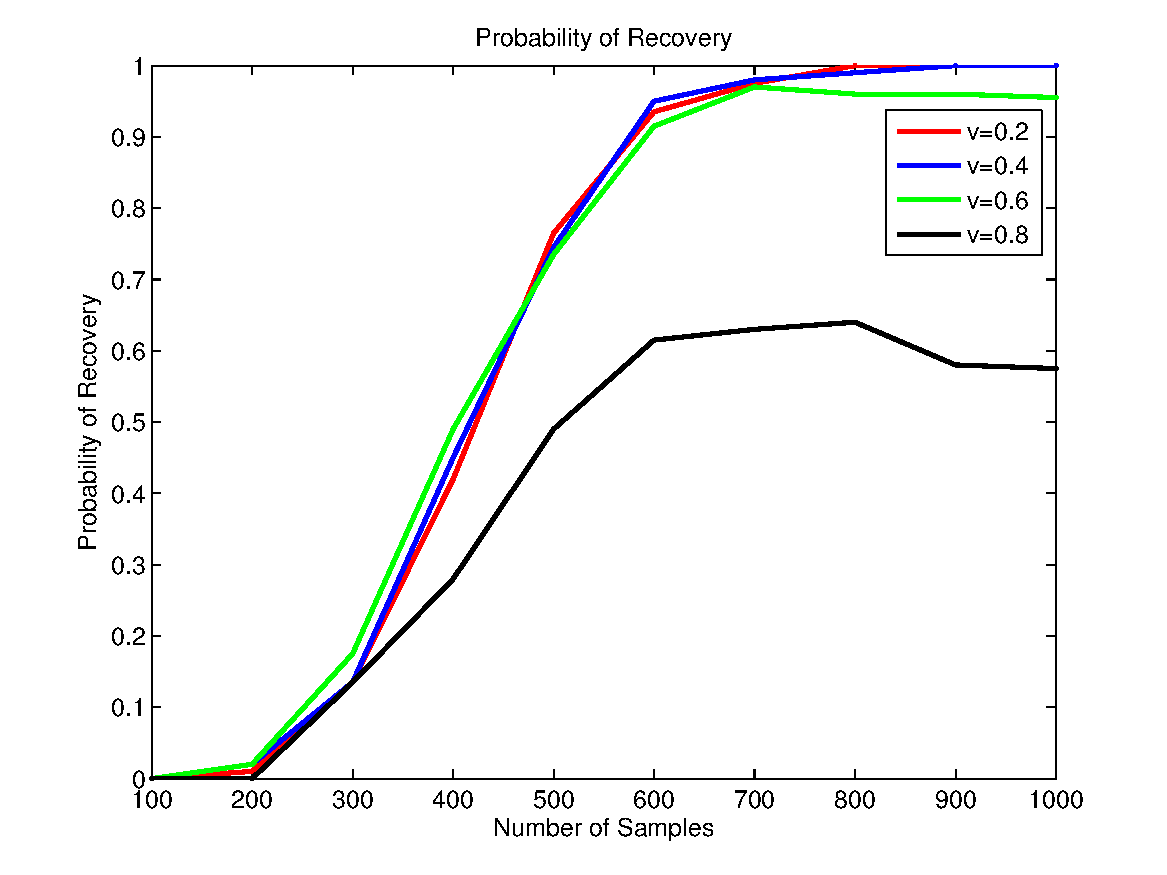
\includegraphics[width=\textwidth]{figs/Curve3}
%                \caption{Correlated design for non-additive model.}
%                \label{Curve3}
%        \end{subfigure}
%        \caption{Result of support recovery.}\label{Support}
%\end{figure}

%\begin{figure}[ht]
%\begin{center}
%\begin{tabular}{cccc}
%\hskip-20pt
%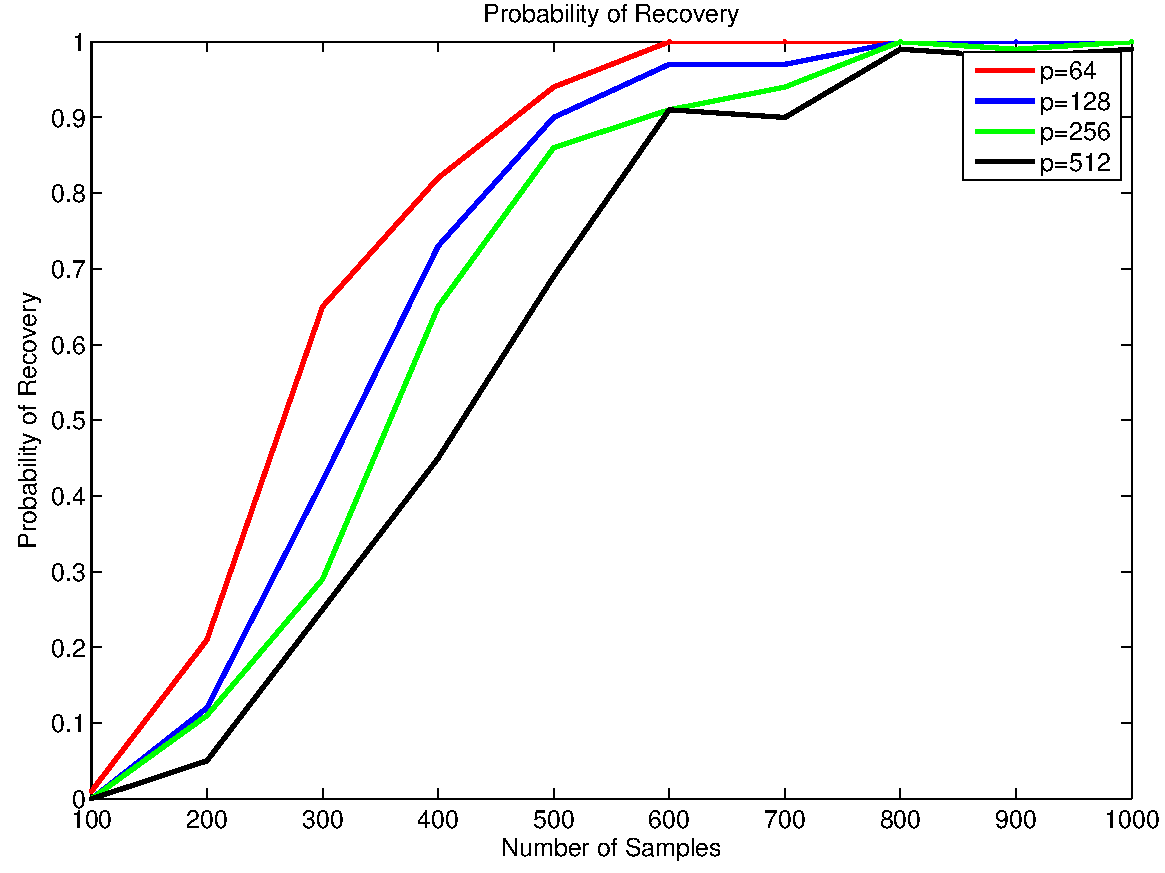
\includegraphics[width=.27\textwidth]{figs/Curve1} &
%\hskip-17pt
%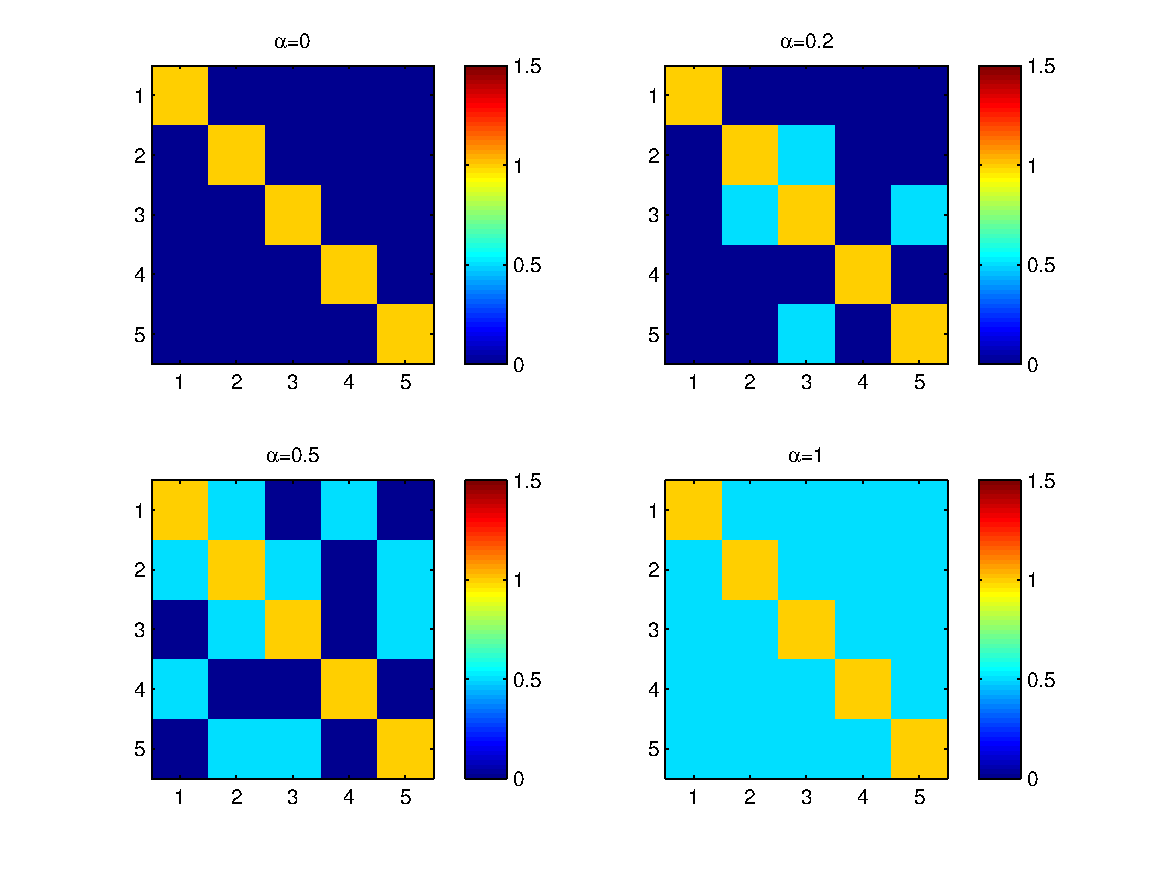
\includegraphics[width=.27\textwidth]{figs/Q} &
%\hskip-17pt
%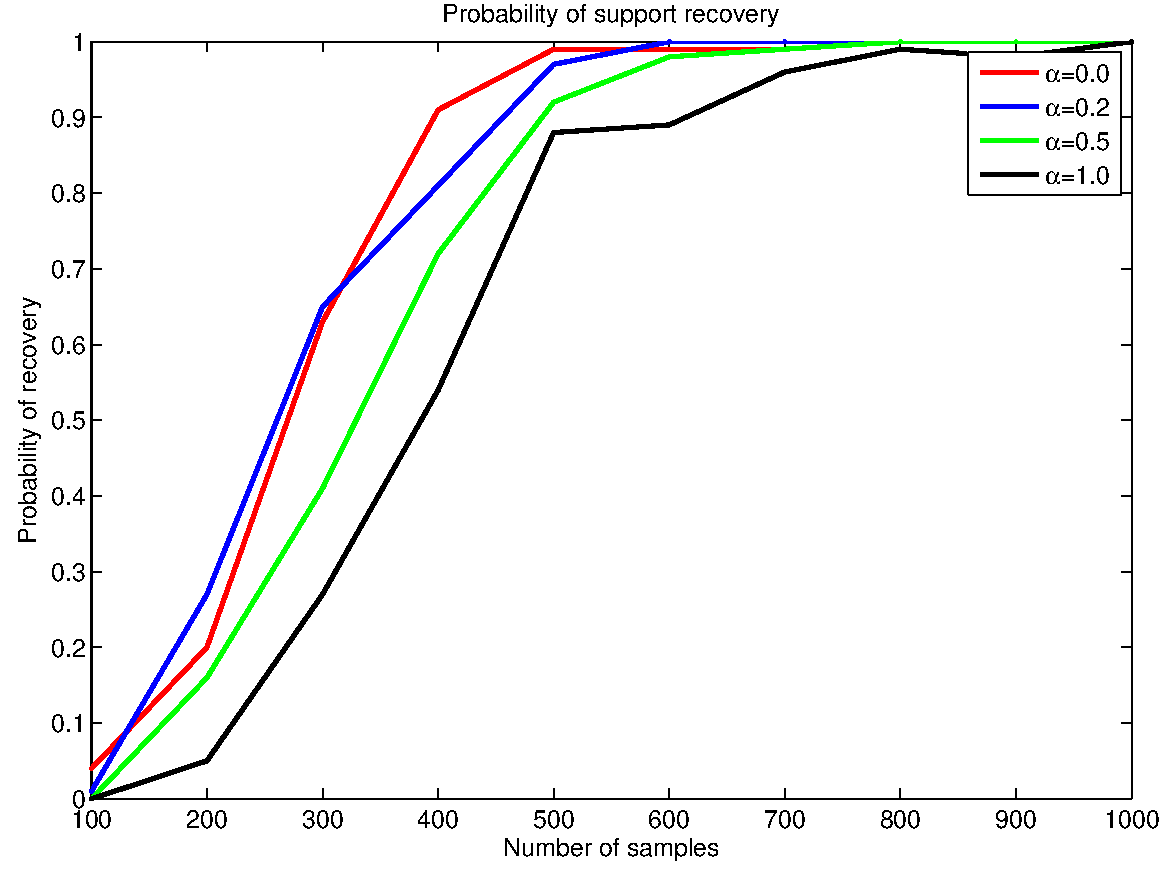
\includegraphics[width=.27\textwidth]{figs/Curve2} &
%\hskip-17pt
%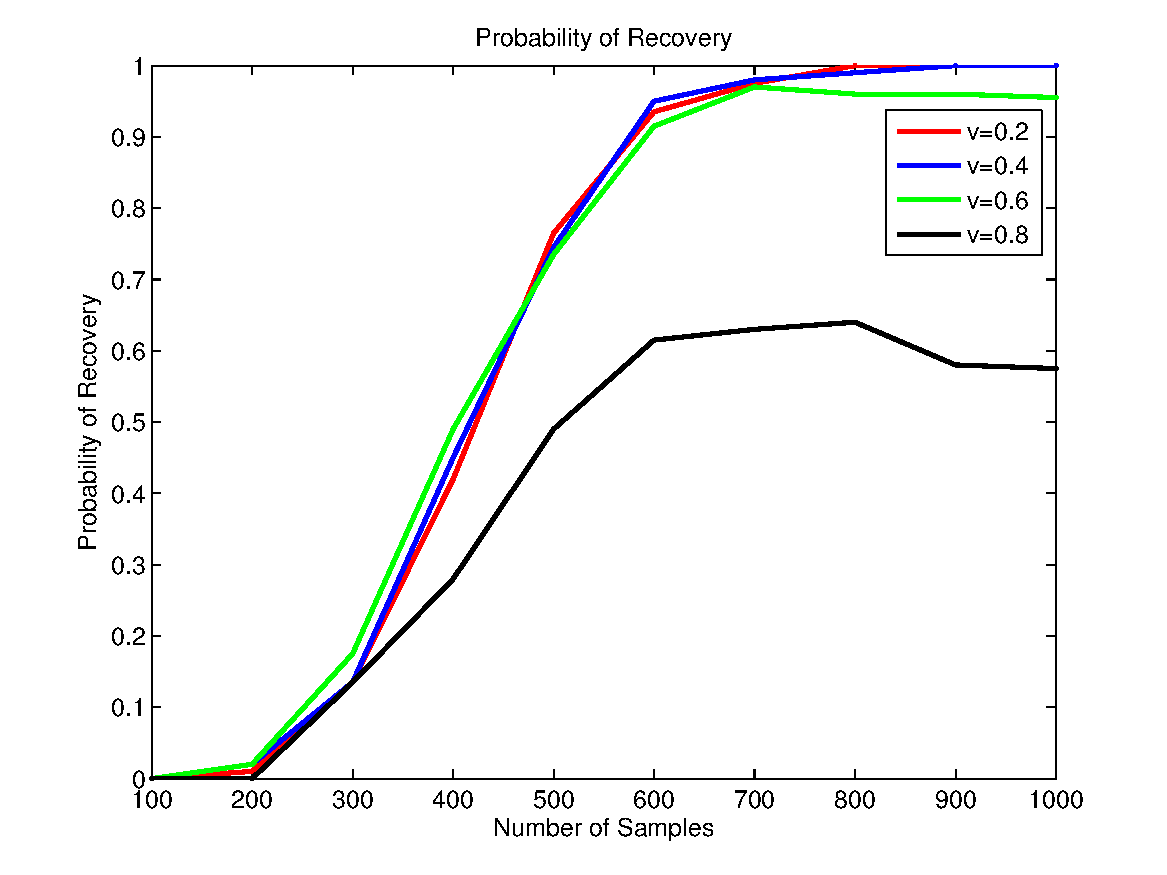
\includegraphics[width=.27\textwidth]{figs/Curve3}  \\
%(a) additive model & (b) four $\Q$ matrices &
%(c) non-additive models & (d) correlated design
%\end{tabular}
%\end{center}
%\caption{Result of support recovery.}\label{Support}
%\end{figure}


%\subsection{Boston housing data}

We next use the Boston housing data rather than simulated data. This data set
contains 13 covariates, 506 samples and one response variable
indicating housing values in suburbs of Boston. The data and detailed description
can be found on the UCI Machine Learning Repository website\footnote{\url{http://archive.ics.uci.edu/ml/datasets/Housing}}. 

We first use all $n=506$ samples (with standardization) in the AC/DC algorithm,
using a set of candidate regularization parameters $\{\lambda^{(t)}\}$
ranging from $\lambda^{(1)} = 0$ (no regularization) to $2$. For each $\lambda^{(t)}$
we obtain a function value matrix $\bds{h}^{(t)}$ with $p=13$
columns. The non-zero columns in this matrix indicate the variables selected
using $\lambda^{(t)}$.  We plot $\|\bds{h}^{(t)}\|_{\infty}$ and
the column-wise mean of $\bds{h}^{(t)}$ versus the normalized norm
$\frac{\|\bds{h}^{(t)}\|_{\infty,1}}{\|\bds{h}^{(1)}\|_{\infty,1}}$
in Figures \ref{Boston}(a) and \ref{Boston}(b).  For comparison, we
plot the LASSO/LARS result in a similar way in Figure \ref{Boston}(c).
From the figures we observe that the first three variables selected by
AC/DC and LASSO are the same: \tts{LSTAT}, \tts{RM} and \tts{PTRATIO},
consistent with previous findings~\citep{SpAM:07}.  The fourth
variable selected by AC/DC is \tts{INDUS} (with $\lambda^{(t)}=0.7$).
We then refit AC/DC with only these four variables without
regularization, and plot the estimated additive functions in Figure
\ref{Boston}(e). When refitting, we constrain a component to be convex if it is non-zero in the AC stage and concave if it is non-zero in the DC stage. As can be seen, these functions contain clear
nonlinear effects which cannot be captured by LASSO. The shapes of
these functions, including the concave shape of the \tts{PTRATIO} function, are in agreement with those obtained by
SpAM~\citep{SpAM:07}. 

Next, in order to quantitatively study the predictive performance, we
run 3 times 5-fold cross validation, following the same procedure
described above---training, variable selection and refitting.  A plot
of the mean and standard deviation of the predictive mean squared
error (MSE) is shown in Figure \ref{Boston}(d). Since for AC/DC the same
regularization level $\lambda^{(t)}$ may lead to a slightly different number of selected
variables in different folds and runs, the values on the $x$-axis
for AC/DC are not necessarily integers. The figure clearly shows that AC/DC has a 
lower predictive MSE than LASSO.  We also compared the performance of
AC/DC with that of Additive Forward Regression (AFR) presented
in~\cite{Xi:09}, and found that they are similar.  The main advantages
of AC/DC compared with AFR and SpAM are that there are no smoothing
parameters required, and the optimization is formulated
as a convex program, guaranteeing a global optimum.

%\begin{figure}[!htpb]
%        \centering
%        \begin{subfigure}[b]{0.45\textwidth}
%                \centering
%                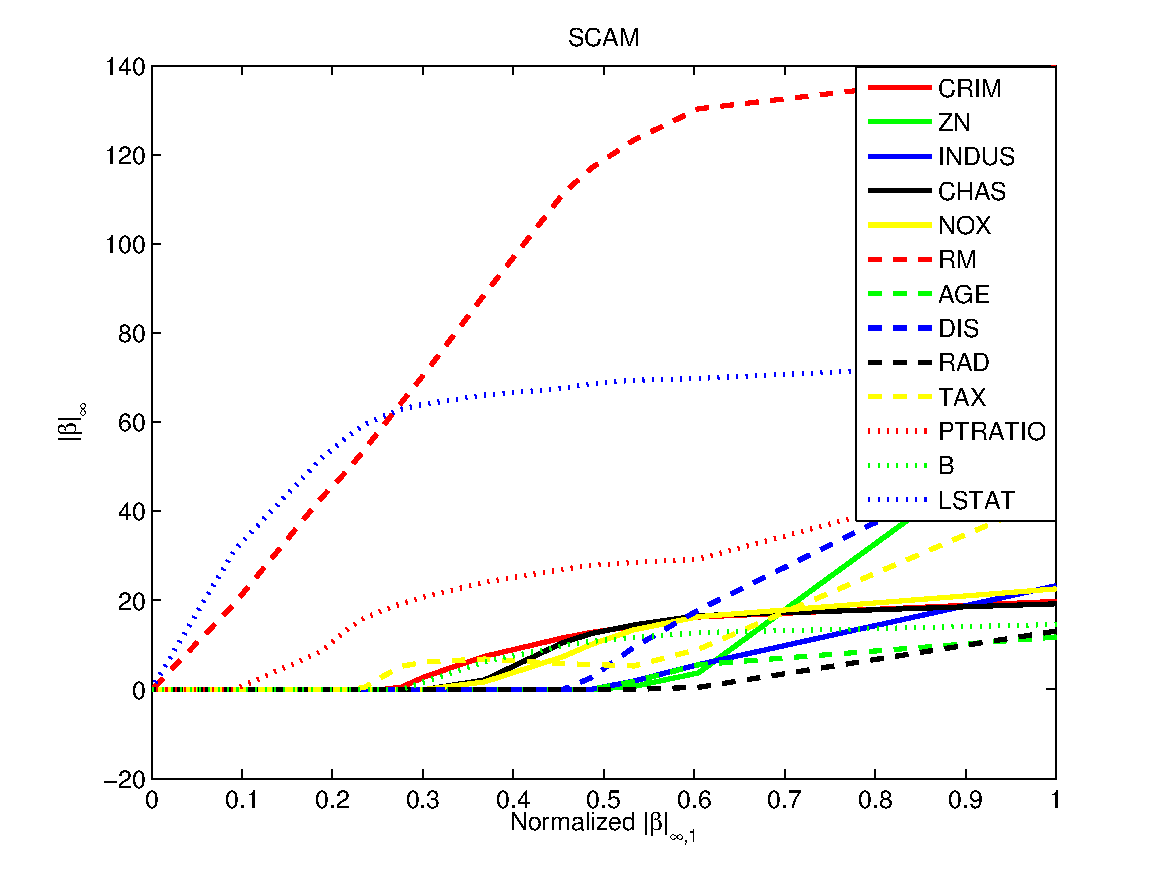
\includegraphics[width=\textwidth]{figs/Additive}
%                 \caption{Variable selection result using AC/DC.}
%                \label{AC/DC}
%        \end{subfigure}
%        \begin{subfigure}[b]{0.45\textwidth}
%                \centering
%                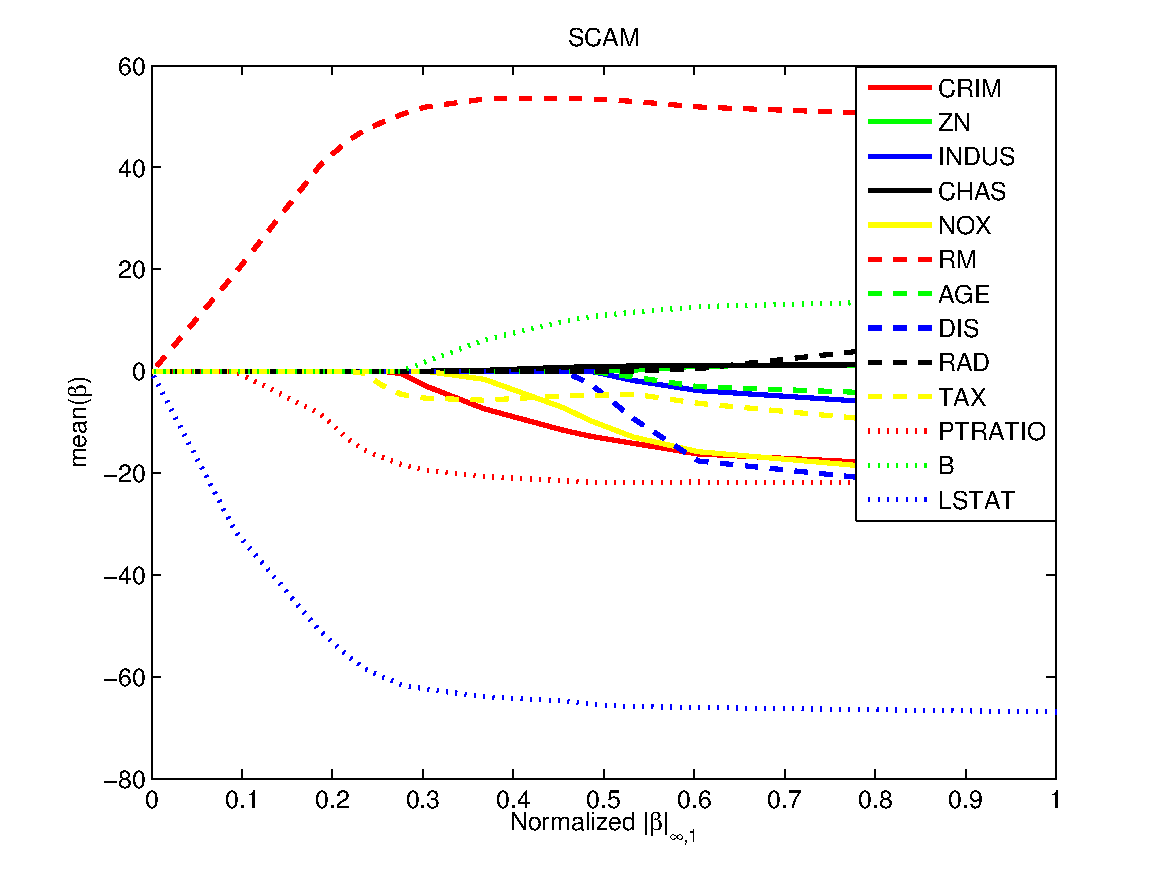
\includegraphics[width=\textwidth]{figs/Additive1}
%                 \caption{Variable selection result using AC/DC.}
%                \label{AC/DC1}
%        \end{subfigure}\\
%        \begin{subfigure}[b]{0.45\textwidth}
%                \centering
%                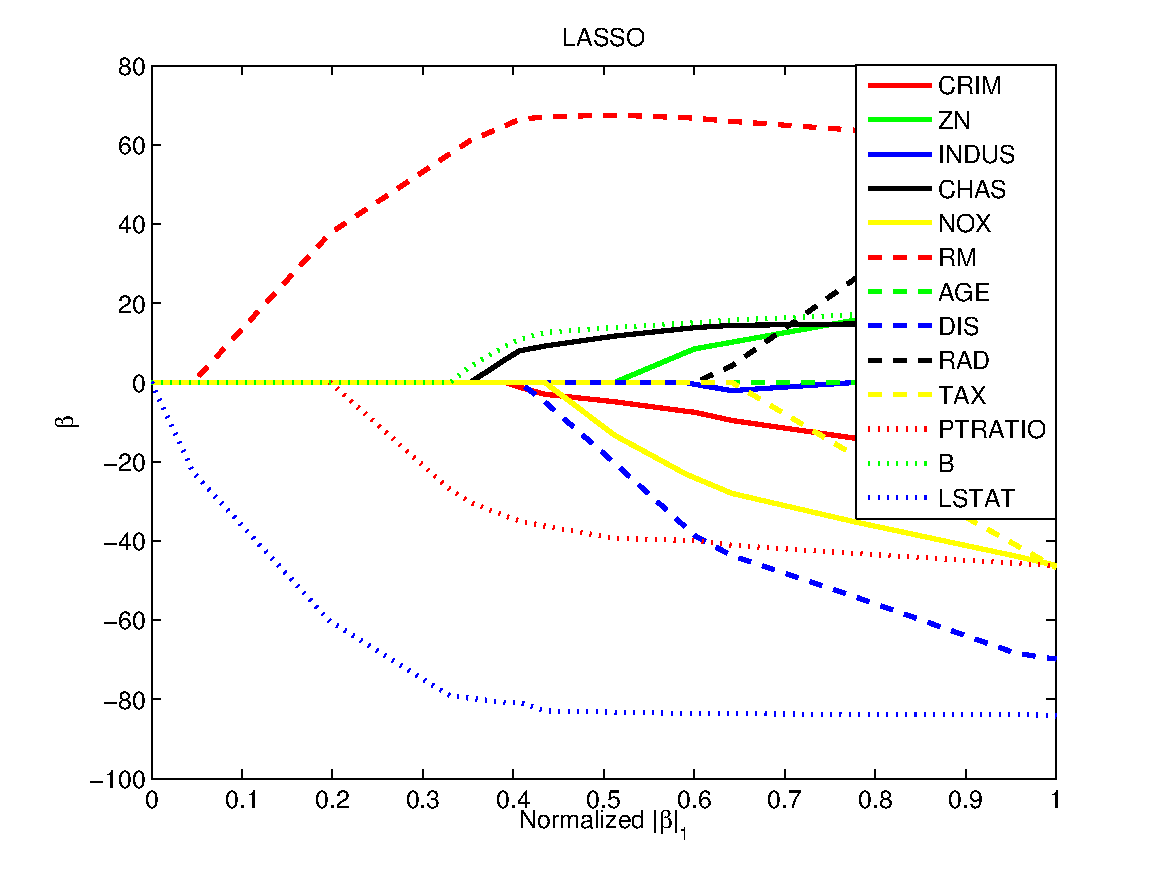
\includegraphics[width=\textwidth]{figs/LASSO}
%                \caption{Variable selection result using LASSO.}
%                \label{LASSO}
%        \end{subfigure}
%        \begin{subfigure}[b]{0.45\textwidth}
%                \centering
%                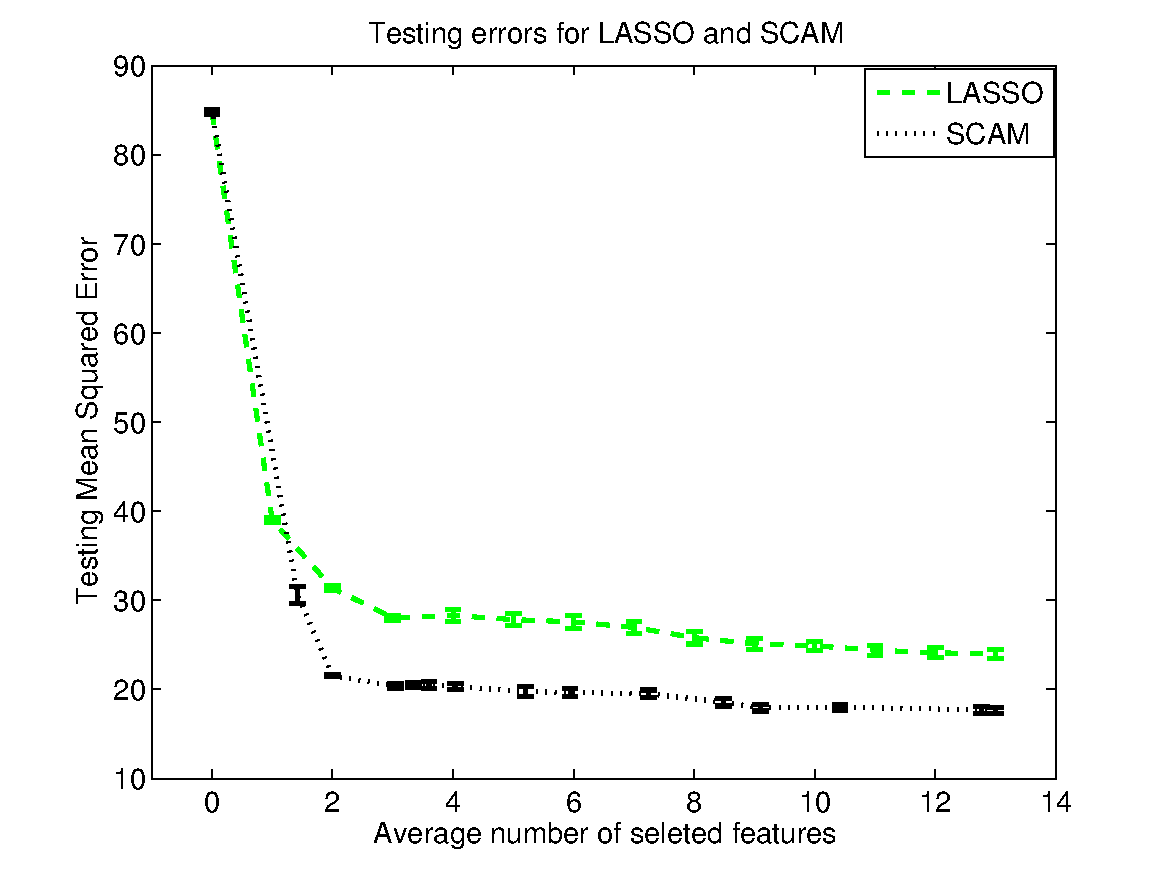
\includegraphics[width=\textwidth]{figs/MSE}
%                 \caption{Predictive MSE of AC/DC and LASSO.}
%                 \label{MSE}
%        \end{subfigure}\\
%        \begin{subfigure}[b]{0.45\textwidth}
%                \centering
%                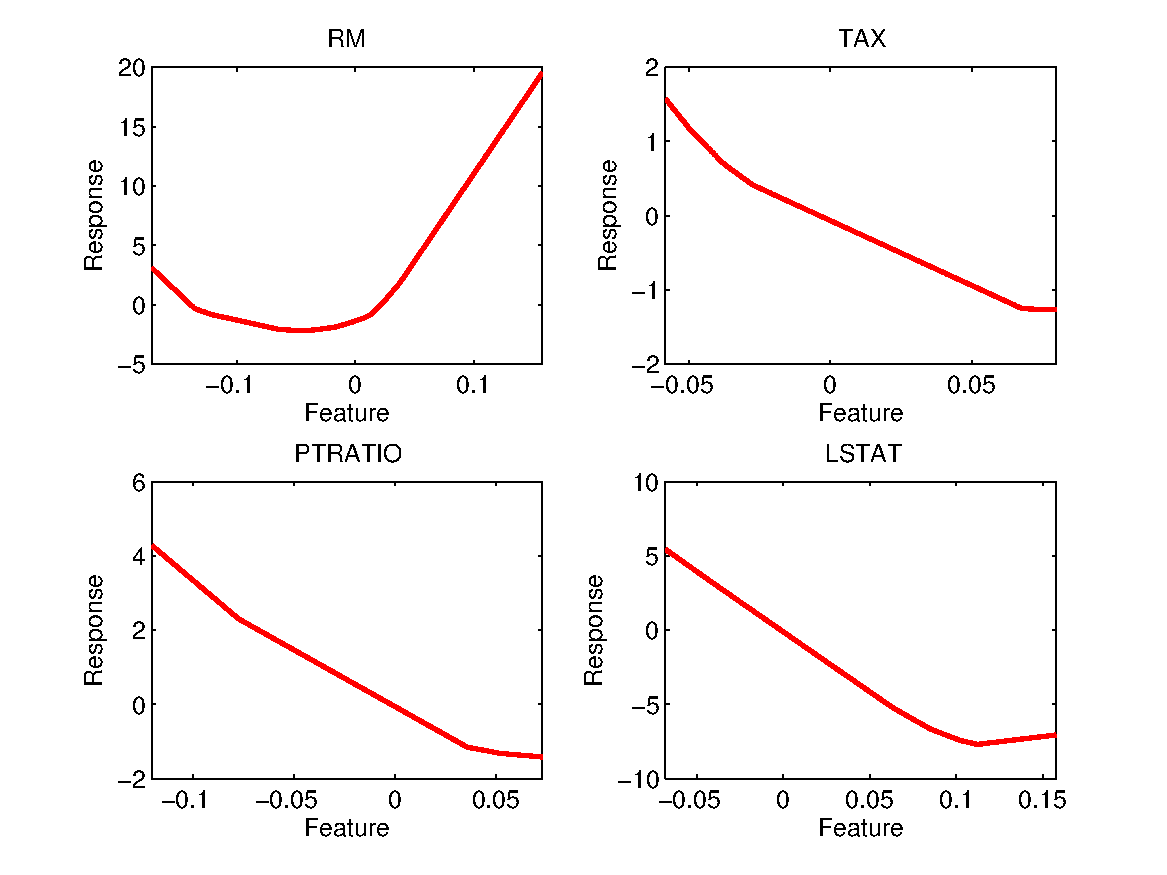
\includegraphics[width=\textwidth]{figs/Convex}
%                \caption{Inferred additive convex functions by AC/DC.}
%                \label{Convex}
%        \end{subfigure}
%        \caption{Results on Boston housing data.}\label{Boston}
%\end{figure}


\begin{figure*}[!t]
\begin{center}
\begin{tabular}{cccc}
\hskip-10pt
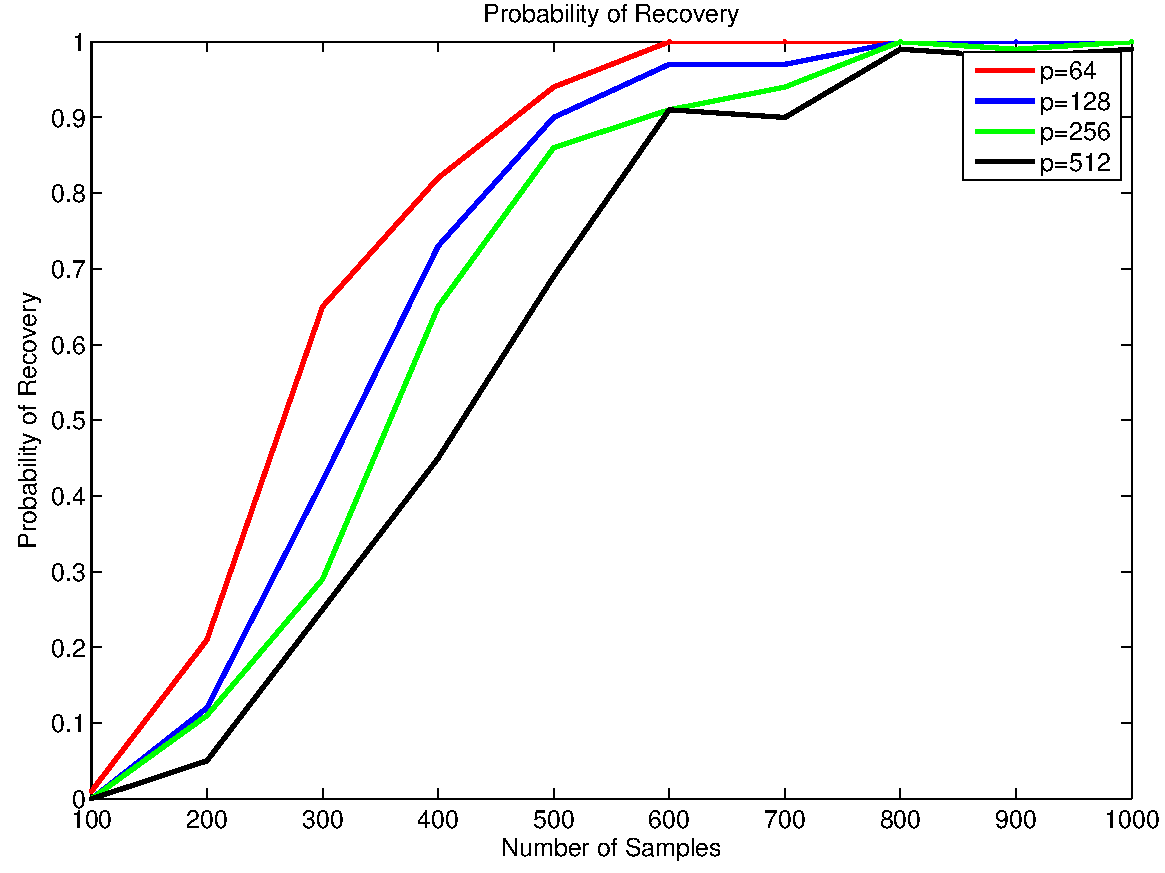
\includegraphics[width=.26\textwidth]{figs/Curve1} &
\hskip-10pt
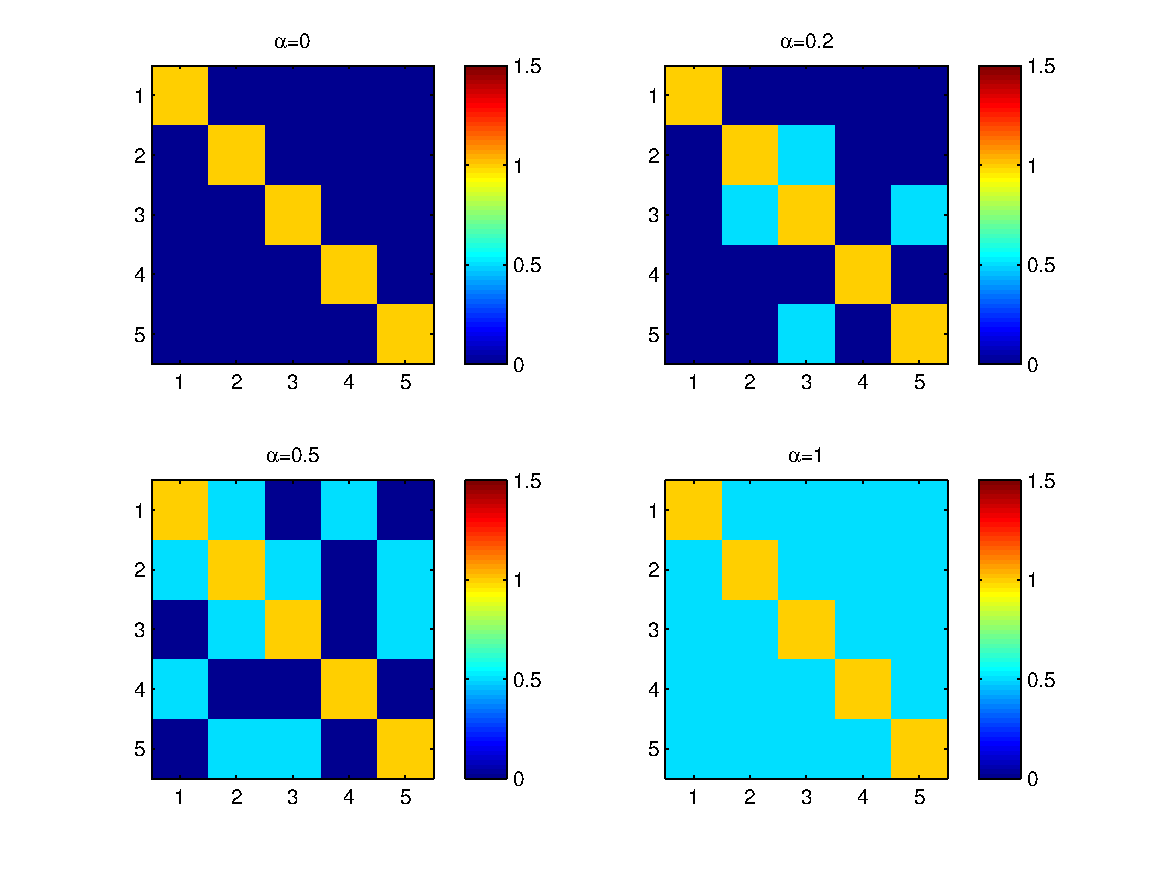
\includegraphics[width=.26\textwidth]{figs/Q} &
\hskip-10pt
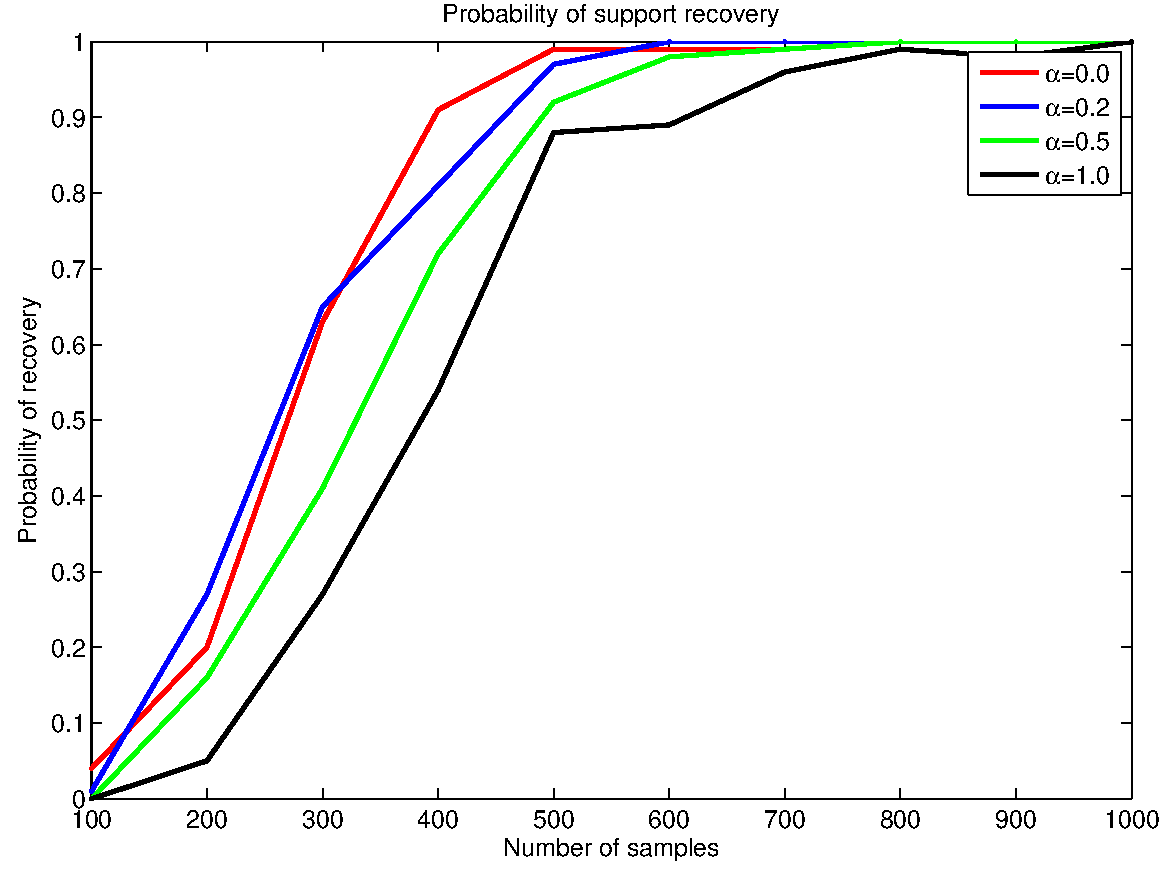
\includegraphics[width=.26\textwidth]{figs/Curve2} &
\hskip-10pt
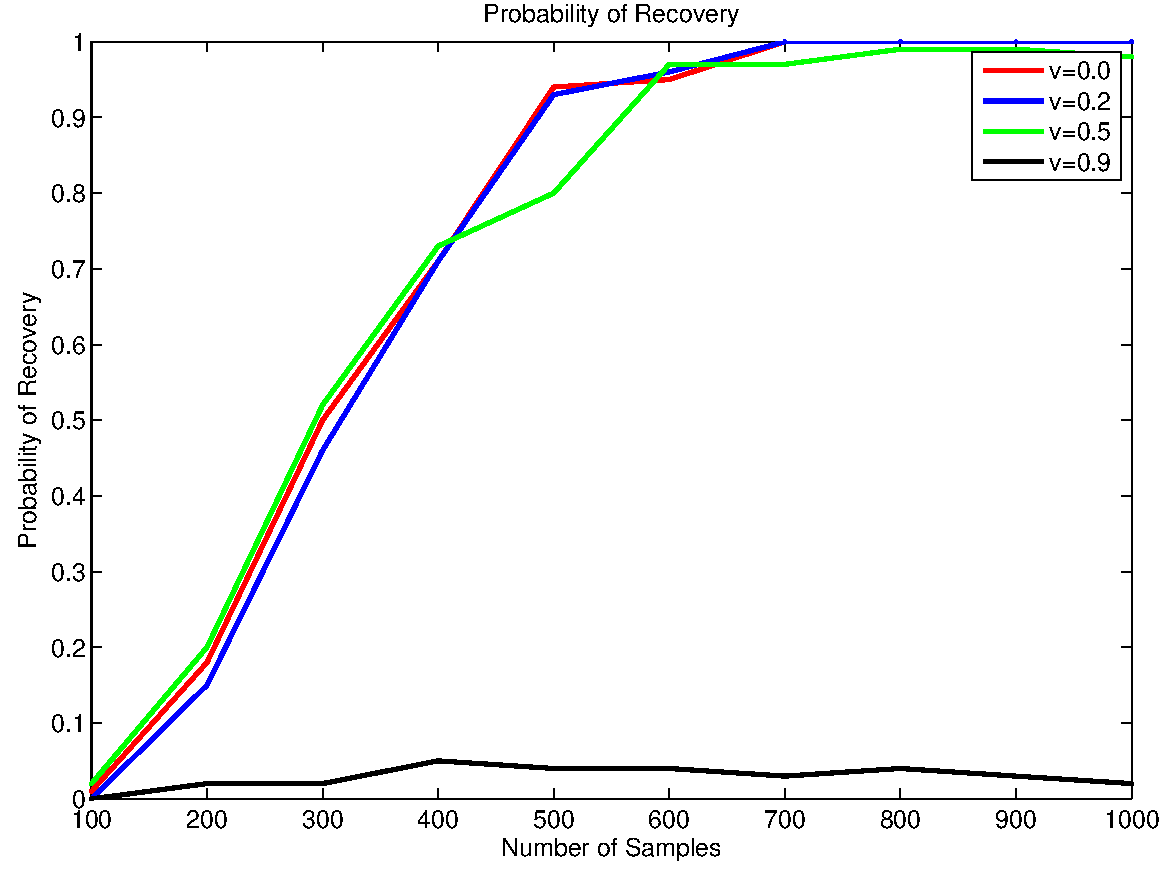
\includegraphics[width=.26\textwidth]{figs/Curve4}  \\
\hskip-10pt (a) additive model & 
\hskip-10pt (b) four $\Q$ matrices &
\hskip-10pt (c) non-additive models & 
\hskip-10pt (d) correlated design
\end{tabular}
\end{center}
\caption{Support recovery results where the additive assumption is
  correct (a), incorrect (b), (c), and with correlated design (d).}\label{Support}
\vskip10pt

\begin{center}
\begin{tabular}{cc}
%\hskip-10pt
  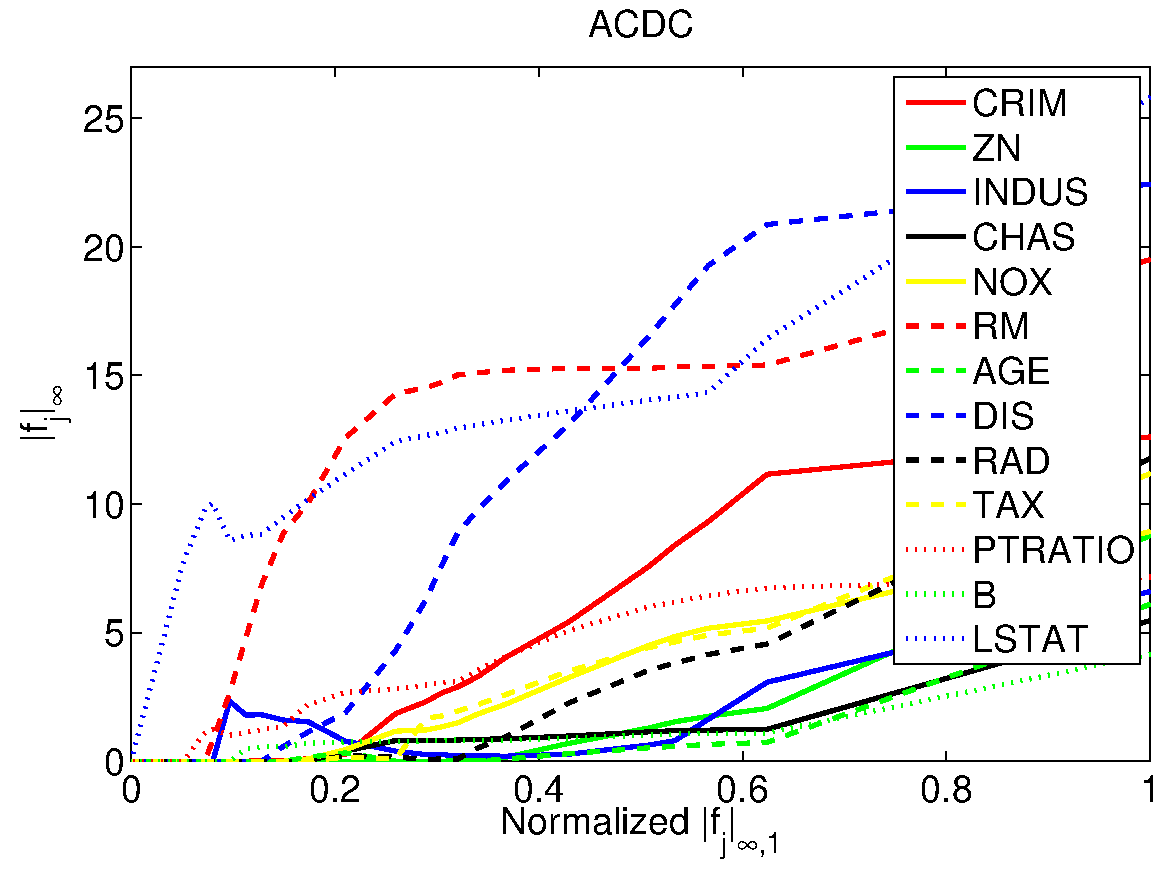
\includegraphics[width=.38\textwidth]{figs/acdc_path} &
%\hskip-25pt
  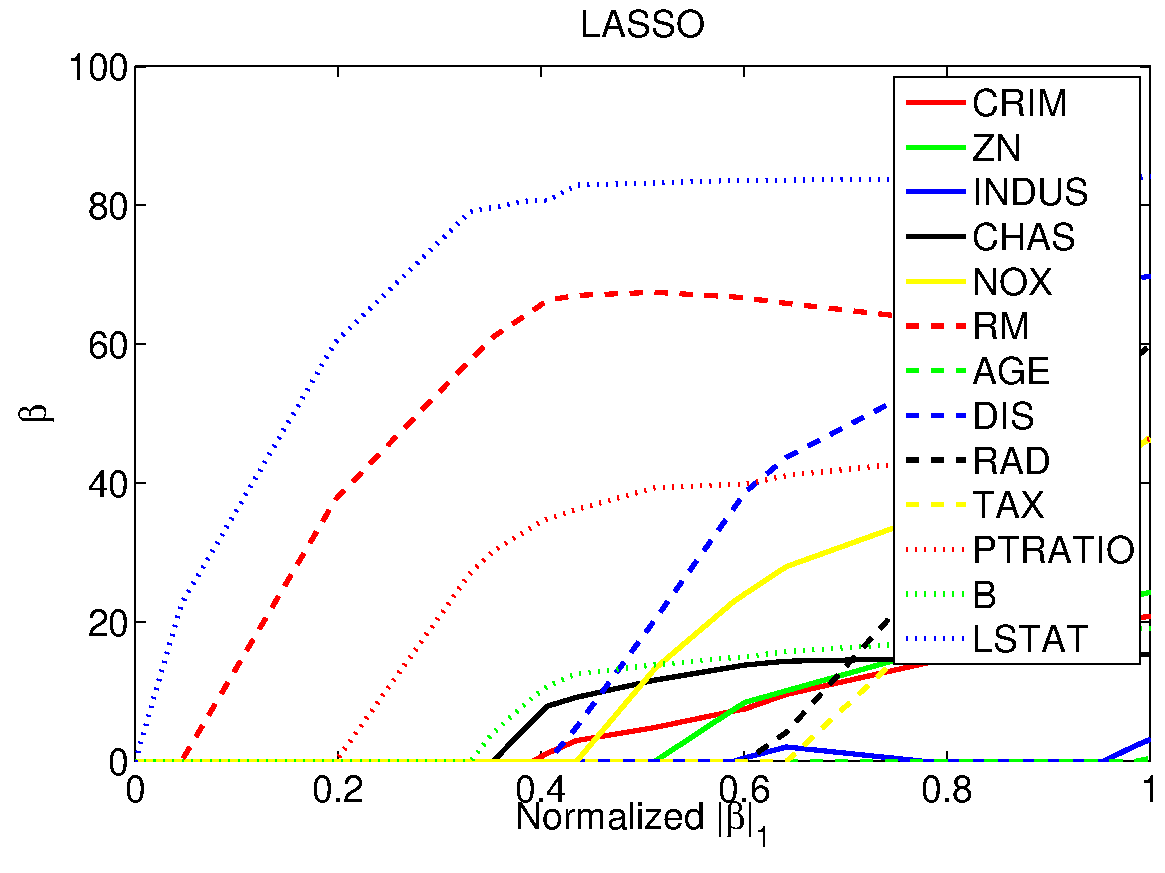
\includegraphics[width=.38\textwidth]{figs/lasso_path} 
\\
%\hskip-10pt 
AC/DC $\|f_k\|_\infty$ paths & 
%\hskip-25pt
LASSO $|\beta_k|$ paths \\
%\end{tabular}
%\begin{tabular}{cc}
  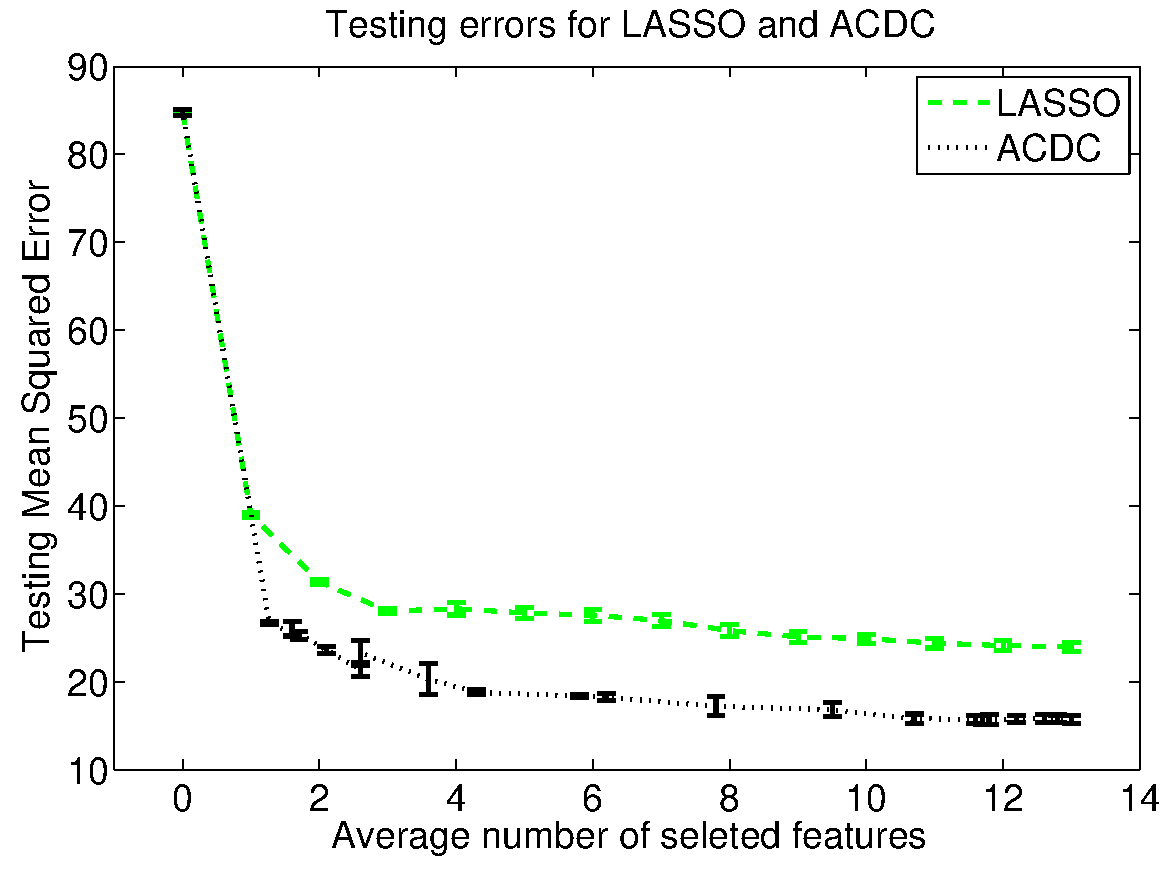
\includegraphics[width=.38\textwidth]{figs/MSEacdc} &
%\hskip 5pt
  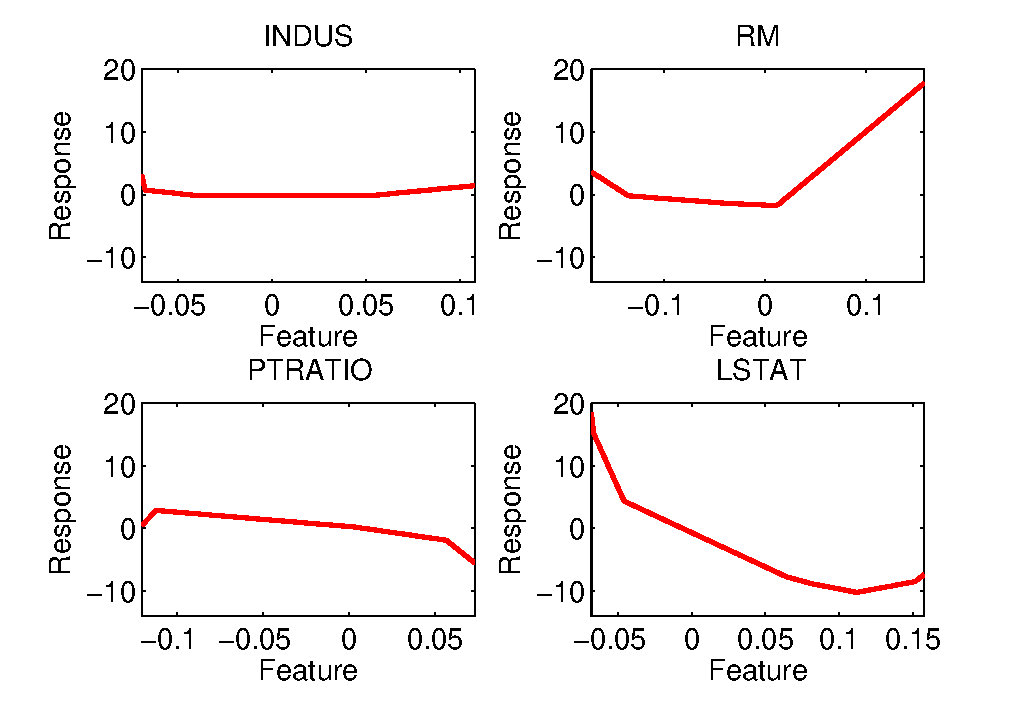
\includegraphics[width=.45\textwidth]{figs/acdc_functs}
\\
predictive MSE & estimated functions from AC/DC
\end{tabular}
\end{center}
\caption{Results on Boston housing data, showing regularization paths,
 MSE and fitted functions.}\label{Boston}
\end{figure*}


% DO NOT CHANGE; RefTex variables -minx
 
%%% Local Variables: ***
%%% mode:latex ***
%%% TeX-master: "paper.tex" ***
%%% End: ***

